%; whizzy chapter
% -initex iniptex -latex platex -format platex -bibtex jbibtex -fmt fmt
% $B0J>e(B whizzytex $B$r;HMQ$9$k>l9g$N@_Dj!#(B


%     Tokyo Debian Meeting resources
%     Copyright (C) 2009 Junichi Uekawa

%     This program is free software; you can redistribute it and/or modify
%     it under the terms of the GNU General Public License as published by
%     the Free Software Foundation; either version 2 of the License, or
%     (at your option) any later version.

%     This program is distributed in the hope that it will be useful,
%     but WITHOUT ANY WARRANTY; without even the implied warranty of
%     MERCHANTABILITY or FITNESS FOR A PARTICULAR PURPOSE.  See the
%     GNU General Public License for more details.

%     You should have received a copy of the GNU General Public License
%     along with this program; if not, write to the Free Software
%     Foundation, Inc., 51 Franklin St, Fifth Floor, Boston, MA  02110-1301 USA

%  preview (shell-command (concat "evince " (replace-regexp-in-string "tex$" "pdf"(buffer-file-name)) "&"))
% $B2hA|%U%!%$%k$r=hM}$9$k$?$a$K$O(Bebb$B$rMxMQ$7$F(Bboundingbox$B$r:n@.!#(B
%(shell-command "cd image200905; ebb *.png")

%%$B$3$3$+$i%X%C%@3+;O!#(B

\documentclass[mingoth,a4paper]{jsarticle}
\usepackage{monthlyreport}

% $BF|IU$rDj5A$9$k!"Kh7nJQ$o$j$^$9!#(B
% date --date 'third saturday'
\newcommand{\debmtgyear}{2009}
\newcommand{\debmtgmonth}{5}
\newcommand{\debmtgdate}{16}
\newcommand{\debmtgnumber}{52}

\begin{document}

\begin{titlepage}
\thispagestyle{empty}

% $B%?%$%H%k%Z!<%8(B:$BJT=8I,MW$JItJ,$O:G=i$N%^%/%m$KHt$P$9$3$H(B

\vspace*{-2cm}
$BBh(B\debmtgnumber{}$B2s(B $BEl5~%(%j%"(B Debian $BJY6/2q;qNA(B

\hspace*{-2.4cm}
\includegraphics[width=210mm]{image200801/2008title.eps}\\
\hfill{}\debmtgyear{}$BG/(B\debmtgmonth{}$B7n(B\debmtgdate{}$BF|(B

\end{titlepage}

\dancersection{Introduction}{$B>e@n(B $B=c0l(B}

\begin{multicols}{2}
 
 
 $B:#7n$N(BDebian$BJY6/2q$X$h$&$3$=!#$3$l$+$i(BDebian$B$N@$3&$K$"$7$rF'$_F~$l$k$H(B
 $B$$$&J}$b!"$9$G$K$I$C$W$j$H$D$+$C$F$$$k$H$$$&J}$b!"7n$K0l2s(BDebian$B$K$D$$(B
 $B$F8l$j$^$;$s$+!)(B

 Debian$BJY6/2q$NL\E*$O2<5-$G$9!#(B

 \begin{itemize}
 \item \underline{Debian Developer} ($B3+H/<T(B)$B$N0i@.!#(B
 \item $BF|K\8l$G$N!V(B\underline{$B3+H/$K4X$9$k>pJs(B}$B!W$r@0M}$7$F$^$H$a!"%"%C%W%G!<%H$9$k!#(B
 \item \underline{$B>l(B}$B$NDs6!!#(B
 \begin{itemize}
  \item $BIaCJ$P$i$P$i$J>l=j$K$$$k?M!9$,(B face-to-face $B$G=P2q$($k>l$rDs6!(B
	$B$9$k!#(B
  \item Debian $B$N$?$a$K$J$k$3$H$r8l$k>l$rDs6!$9$k!#(B
  \item Debian$B$K$D$$$F8l$k>l$rDs6!$9$k!#(B
 \end{itemize}
 \end{itemize}		

 Debian$B$NJY6/2q$H$$$&$3$H$G5f6KE*$K$O;22C<TA40w$,(BDebian Package$B$r$,$j$,$j(B
 $B$H:n$k%9!<%Q!<%O%C%+!<$K$J$C$?;Q$rLQA[$7$F$$$^$9!#>pJs$N6&M-!&3hMQ$rDL$7(B
 $B$F(B Debian$B$N:#8e$NG=F0E*$JE83+$X$NEZBf$H$7$F!"!V>l!W$H$7$F$N6u4V$rDs6!$9(B
 $B$k$N$,L\E*$G$9!#(B

 2009$BG/$N7W2h$O2>$G$9!#(B

 \begin{enumerate}
  \item $B?7G/$N4k2h(B ($B%"%s%5%s%V%k2.7&3+:E(B)
  \item OSC Tokyo
  \item VAIO P $B%$%s%9%H!<%k5-O?!"(B
	$B%+!<%M%kFI=q2q!!%G%#%9%H%j%S%e!<%7%g%sBg=89g(B($B>.NS$5$s(B)($BEl5~Bg3X(B?)
  \item Git Handson ($B4d>>(B)($B$"$s$5$s$V$k2.7&(B?)
  \item $B2H(BDebian$B%5!<%P(B vs $B?&>l$N%M%C%H%o!<%/(B($B@iBeED6hETN)?^=q4[(B?\footnote{\url{http://www.library.chiyoda.tokyo.jp/}})
  \item Asterisk ($BEl5~Bg3X(B?)
  \item $B%9%Z%$%s$K$F3+:E(B
  \item Debconf$BJs9p2q(B
  \item OSC Fall?
  \item udev + HAL($B4d>>$5$s(B)
  \item 3D graphics $B3+H/!JF#Bt$5$s!K(B 
  \item Debian $B%5!<%P(B+VMware + $B3F<o(BOS$B!"(B
	$BB>$N2>A[2=%D!<%k(B(vserver etc.)$B!"(B
	$BK:G/2q(B
 \end{enumerate}

 $B2q>l8uJd$H$7$F$O2<5-$,$"$j$^$9(B:

 \begin{itemize}
  \item $BBg3X(B
  \item $B7CHf<w(BSGI$B%[!<%k(B
  \item Google$B%*%U%#%9(B
  \item $B8xL14[(B($B$"$s$5$s$V$k2.7&Ey(B)
  \item $BETN)2q5D<<(B($BL5@~(BLAN)
  \item $B7rJ]$N;\@_(B
 \end{itemize}

\end{multicols}


\newpage

\begin{minipage}[b]{0.2\hsize}
 \definecolor{titleback}{gray}{0.9}
 \colorbox{titleback}{\rotatebox{90}{\fontsize{80}{80} {\gt $B%G%S%"%sJY6/2q(B} }}
\end{minipage}
\begin{minipage}[b]{0.8\hsize}
\hrule
\vspace{2mm}
\hrule

\setcounter{tocdepth}{2}
\tableofcontents
\vspace{2mm}
\hrule
\end{minipage}

\dancersection{$B;vA02]Bj(B}{$B>e@n(B $B=c0l(B}

$B;vA02]Bj$O(B:

\begin{enumerate}
 \item xxx
\end{enumerate}

$B$3$N2]Bj$KBP$7$FDs=P$$$?$@$$$?FbMF$O0J2<$G$9!#(B

\begin{multicols}{2}
%; whizzy-master ../debianmeetingresume200905.tex
% $B0J>e$N@_Dj$r$7$F$$$k$?$a!"$3$N%U%!%$%k$G(B M-x whizzytex $B$9$k$H!"(Bwhizzytex$B$,MxMQ$G$-$^$9!#(B

\begin{prework}{$B>e@n=c0l(B}

\preworksection{$BE,MQ$7$?<gMW$JJ}K!(B}

DDTSS $B$r%V%i%&%6$GD/$a$F!"K]Lu$r%l%S%e!<$7$F$_$^$7$?!#(B
$B%Q%C%1!<%8$N(Bdescription$B$@$1$GJ,$+$i$J$$ItJ,$K$D$$$F$O%P%0%l%]!<%H$r$7$^(B
$B$7$?!#(B
$BITL@E@$O(B debian-doc@jp $B%a!<%j%s%0%j%9%H$K<ALd$H$7$FEj9F$7$^$7$?!#(B

\preworksection{$BH/8+$7$?2]Bj(B}

$B%l%S%e!<$r$7$FJ,$+$C$?$3$H$G$9$,!"K]Lu$N:n6H$GC18l$NK]Lu$^$G$O$G$-$F$$$k(B
$B$N$G$9$,!"J8>OA4BN$H$7$F78$j<u$1$,$*$+$7$/!"0UL#$,DL$C$F$$$J$$$b$N$,$"$j$^$7$?!#(B
$B$^$?!"1Q8l$N6gFIE@$r$=$N$^$^F|K\8l$N6gFIE@$KCV$-49$($F$*$j!"$=$N$^$^$G$OF|K\8l$H$7$F(B
$BJ8>O$,D9$9$.$k$b$N$b$"$j$^$7$?!#K]Lu:n6H$rD>Lu:n6H$H$9$k$HFI$_$K$/$$(B
Description$B$,$G$-$"$,$C$F$7$^$&$H;W$o$l$^$9!#(B

\preworksection{$BDs0F$9$kM}A[A|(B($B%D!<%k$H$+(B)$B!"6&M-$7$?$$>pJs(B}

\begin{itemize}
 \item Description $B$KBP$7$F$9$G$K%P%0%l%]!<%H$,Ej9F$5$l$F$$$k$+$I$&$+$N(B
       $B%A%'%C%/$9$k%D!<%k!#(B

 \item $BMQ8l=8$K$9$G$K7G:\$5$l$F$$$kMQ8l$r4JC1$K%&%'%V%V%i%&%6$+$i%A%'%C%/(B
       $B$G$-$k(Bgreasemonkey $B!#(B

 \item DDTSS $B$G9T$C$?%l%S%e!<!&%3%a%s%H$J$I$,(B debian-doc@jp $B%a!<%j%s%0%j(B
       $B%9%H$KH?1G$9$k$3$H!#(B
\end{itemize}

\end{prework}

\begin{prework}{$B$^$($@$3$&$X$$(B}
\preworksection{$BE,MQ$7$?<gMW$JJ}K!(B}
$B;vA02]Bj$^$G<j$,2s$i$:$8$^$$!#$@$1$@$H7]$,$J$$$N$G!"8=:_M'?M$H?J$a$F$$$k(B
 CouchDB$B$N(BWeb$B%5%$%H$NK]Lu$K$D$$$FOC$7$^$9!#(B
\begin{enumerate}
 \item CouchDB$B$N(BWeb$B%5%$%H$r(BGoogle Docs$B$G$^$k$4$H<h$j9~$`!##1%Z!<%8$K$D$-!"(B
       $BK]Lu<T$O8BDj!#B>$O::FI$7!"0lJ8$:$DK]Lu$9$k!#D>Lu$G$O$J$/!"F|K\8l(B
       $B$H$7$F$o$+$j$d$9$$J8>O$r=E;k!#(B
 \item Web$B%5%$%H!"(BWiki$B$r$"$kDxEY$NHfN($^$GK]Lu$r?J$a$k!#(B
 \item CouchDB$B$N3+H/<T8~$1$N(BML$B$K8x3+$7$?$$;]$rAjCL$9$k!#(B
 \item Debian$B$N(BCouchDB$B$N%Q%C%1!<%8%a%s%F%J$G$b$"$k!"3+H/<T$+$i(Bpo4a$B$r;H$&(B
       $B$3$H!"B>$K$b$$$m$$$m2]Bj!J%7%9%F%`4IM}!"%"%C%W%m!<%I$NJ}K!!"K]Lu(B
       $B$NDDIe2=$J$I!K$,$"$k$1$I$=$l$r9MN8$7$J$$$H$$$1$J$$$h$H!"%"%I%P%$(B
       $B%9$r$b$i$&!#(B
 \item PO$B7A<0$G%Q%C%AEj$2$FH?1G<+BN$O$*4j$$$7!"99?7$O$J$s$i$+$N<jCJ$G3N(B
       $BG'$7$F?o;~K]Lu$7$F$$$/;]$rEA$($k!#(B
 \item $B:#8e$NJ}?K$r$I$&$9$k$+$rM'?M$HAjCL$7$F!":#%3%3!#(B
\end{enumerate}

\preworksection{$BH/8+$7$?2]Bj(B}
Web$B%5%$%H$O(BXHTML$B$K$J$C$F$$$J$$$N$G!"$^$:JQ49$9$k$H$3$m$+$i;O$a$J$$$H$$$1(B
 $B$J$$$3$H$H!"(BWiki$B$O99?7$,IQHK$K$"$j$9$.$@$+$i!"BP>]$+$i30$7$?J}$,NI$$$h(B
 $B$M!"$HM'?M$HAjCL$7$?$H$3$m!#K]Lu$,$=$b$=$b$d$j$?$$$3$H$G$O$J$+$C$?$N$G!#(B

\preworksection{$BDs0F$9$kM}A[A|(B($B%D!<%k$H$+(B)$B!"6&M-$7$?$$>pJs(B}
$B:G=i$NK]Lu$@$19T$C$?$i!"8e$O<jN%$l$9$k!JC/$+$K0z$-7Q$0!K$N$,M}A[$G$O$"$k(B
 $B$b$N$N!"6(NO<T$rA}$d$5$J$$$H$$$1$J$$!#$=$b$=$b(BDebian$B%Q%C%1!<%8$K$J$C$F(B
 $B$$$k$N$G!"%=!<%9%Q%C%1!<%8$K4^$^$l$k%I%-%e%a%s%H$J$i!"(BDebian-doc$B$GK]Lu(B
 $B$7$F!"$=$C$A7PM3$G%"%C%W%9%H%j!<%`$KH?1G$7$F$b$i$&!"$H$$$&$N$b<j$@$J$H(B
 $B$$$&$3$H$r8!F$Cf!#(B
\end{prework}

\begin{prework}{$B$"$1$I(B}

$B@bL@J8$rK]Lu$7$?%Q%C%1!<%8(B
libvolpack1	$B%l%s%@%j%s%0%i%$%V%i%j(B
libvolpack1-dev	$B%l%s%@%j%s%0%i%$%V%i%j(B
nagios3		$B%7%9%F%`4F;k(B/$B4IM}%D!<%k(B
nagios3-doc	$B%7%9%F%`4F;k(B/$B4IM}%D!<%k$NJ8=q(B
cwcp		$B%b!<%k%9?.9fN}=,%=%U%H(B
dnswalk		DNS$B%A%'%C%/%D!<%k(B
slapd		LDAP$B%5!<%P(B
pingpong	$B%"%^%A%e%"L5@~MQ(B convers $B%5!<%P(B
sugar-presence-service	OLPC$BMQ%=%U%H(B
amap-align	DNA$B2r@O%D!<%k(B
loki		DNA$B2r@O%D!<%k(B
xastir		DNA$B2r@O%D!<%k(B
biosquid	DNA$B2r@O%D!<%k(B
boxshade	DNA$B2r@O%D!<%k(B
dialign		DNA$B2r@O%D!<%k(B
dialign-t	DNA$B2r@O%D!<%k(B
probcon		DNA$B2r@O%D!<%k(B

$B!A%l%S%e!<$3$3$+$i!A(B
$B%l%S%e!<(B 1
$B%Q%C%1!<%8(B: libvolpack1

Short description
$B86J8(B: fast volume rendering library
$BLuJ8(B: $B9bB.$JBgNL%l%s%@%j%s%0%i%$%V%i%j(B

Long description
$B86J8(B:
VolPack is a software library for fast, high-quality volume rendering with
this features:
 * Renders data sampled on a regular, three-dimensional grid.
 * Supports user-specified transfer functions for both opacity and color.
 * Provides a shading model with directional light sources, multiple material
   types with different reflective properties, depth cueing, and shadows.
 * Produces color (24 bits/pixel) or grayscale (8 bits/pixel) renderings,
   with or without an alpha channel.
 * Supports arbitrary affine view transformations.
 * Supports a flexible data format that allows an arbitrary C structure to be
   associated with each voxel.
$BLuJ8(B:
VolPack $B$O9bIJ<A$G9bB.$JBgNL$N%l%s%@%j%s%0$r9T$&%=%U%H%&%'%"%i%$%V%i%j$G!"(B
$B<!$NMM$JFCD'$r;}$C$F$$$^$9(B:
 * $B@55,2=$5$l$?%5%s%W%k%G!<%?$r(B 3 $B<!85%0%j%C%I$KI=<((B
 * $BITF)L@$H%+%i!<N>J}$N%f!<%6Dj5A$NJQ494X?t$r%5%]!<%H(B
 * $BJ}8~;XDj$5$l$?8w8;$K$h$k1"1FIU$-%b%G%k!"0c$&H?<MFC@-$r;}$C$?J#?t$NAG:`%?(B
   $B%$%W!"G;C8!"5Z$S1F$rDs6!(B
 * $B%"%k%U%!%A%c%M%k$NM-$j!"L5$7$N(B (24 $B%S%C%H(B/$B2hAG$N(B) $B%+%i!<$^$?$O(B (8 $B%S%C%H(B
   /$B2hAG$N(B) $B%0%l!<%9%1!<%9$G$NIA2h$N@8@.(B
 * $BG$0U$N;kE@$N%"%U%#%sJQ49$r%5%]!<%H(B
 * $BG$0U$N(B C $B8@8lE*$J9=B$$r%\%/%;%k(B (3 $B<!853J;R>e$N:G>.N)J}BN!"(B2 $B<!85$G$N(B
   $B%T%/%;%k(B) $B$X7k$S$D$1$k;v$,=PMh$k=@Fp$J%G!<%?%U%)!<%^%C%H$N%5%]!<%H(B

$B%l%S%e!<(B 2
$B%Q%C%1!<%8(B: amap-align

Short description
$B86J8(B: Protein multiple alignment by sequence annealing
$BLuJ8(B: $B%7!<%/%(%s%9%"%K!<%j%s%0$K$h$kCAGr<A$N%^%k%A%W%k%"%i%$%a%s%H(B ($BB?=EG[Ns@0Ns(B)

Long description
$B86J8(B:
AMAP is a command line tool to perform multiple alignment of peptidic
sequences. It utilizes posterior decoding, and a sequence-annealing
alignment, instead of the traditional progressive alignment method. It
is the only alignment program that allows to control the sensitivity /
specificity tradeoff.  It is based on the ProbCons source code, but
uses alignment metric accuracy and eliminates the consistency
transformation.
.
 Homepage: http://bio.math.berkeley.edu/amap/
$BLuJ8(B:
AMAP $B$O%Z%W%A%IG[Ns$N%^%k%A%W%k%"%i%$%a%s%H(B ($BB?=EG[Ns@0Ns(B) $B$r9T$&%3%^%s%I(B
$B%i%$%s%D!<%k$G$9!#;v8e2rFI$KMxMQ$5$l!"EAE}E*$J%W%m%0%l%C%7%V%"%i%$%a%s%H(B
$BK!$NBe$o$j$K%7!<%/%(%s%9%"%K!<%j%s%0$N@0Ns$r9T$$$^$9!#46EY(B \& $BFC0[@-$N(B
$B%H%l!<%I%*%U$r%3%s%H%m!<%k=PMh$kM#0l$N%"%i%$%a%s%H(B ($B@0Ns(B) $B%W%m%0%i%`$G$9!#(B
ProbCons $B$N%=!<%9%3!<%I$r85$K$7$F!"@:L)B,Dj%"%i%$%a%s%H(B ($B@0Ns(B) $B$H%3%s%7(B
$B%9%F%s%7!<%H%i%s%9%U%)!<%a!<%7%g%s(B ($B0l4S@-JQ2=(B) $B$N=|5n$rMxMQ$7$F$$$^$9!#(B
.
 Homepage: http://bio.math.berkeley.edu/amap/

$B!A%l%S%e!<$3$3$^$G!A(B

1$B!#E,MQ$7$?<gMW$JJ}K!(B
$B<jF~NO$H%M%C%H>e$N1QOB<-E5!"I,MW$K1~$8$F(B Google$B!"(Bwikipedia$B!"$=$NB>@lLg%5%$%H$r;2>H(B

2$B!#H/8+$7$?2]Bj(B
DNA$B2r@O%D!<%k$,B?$/$"$j!"@lLgMQ8l$,$^$A$^$A$G(B
$B$=$l$NE}0l<c$7$/$O6&DL2=$,I,MW$@$H;W$$$^$7$?!#(B

3$B!#Ds0F$9$kM}A[A|(B($B%D!<%k$H$+(B)
$B@lLgMQ8l$K$D$$$F$O<-=q%Z!<%8$rMQ0U$9$k$+!"4p=`$K$9$k@lLgMQ8l$N%5%$%H$r7h$a$k$N$,NI$$$+$H;W$$$^$9!#(B

$B!&6&M-$7$?$$>pJs$r@bL@(B
Debian $B%Q%C%1!<%8$K$O?tB?$/$N(B DNA $B2r@O%D!<%k$,$"$C$F!"@lLgMQ8l$NK]Lu$K$"$?$C$FCm0U?<$/:n6H$9$kI,MW$,$"$k$H;W$$$^$9!#(B
DNA $B2r@O$K$D$$$FM=HwCN<1$H$7$F2<5-%5%$%H$,;29M$K$J$k$+$H;W$$$^$9!#(B
$B%?%s%Q%/<A!?3K;@$N%"%i%$%a%s%H2r@O(B 
http://www.icot.or.jp/ARCHIVE/Museum/SOFTWARE/GIP/gene\_alignment.html
$B"(J8;z%3!<%I$,(B ISO-2022-JP $B$J$N$K%(%s%3!<%I>pJs$O(B Shift-JIS $B$K$J$C$F$$$^$9!#(B

Debian JP $BJ8=q:n@.$N;X?K(B $B$K$D$$$F(B DDTSS for ja $B$K%j%s%/$,$"$C$?J}$,NI$$$+$H;W$$$^$9!#(B

\end{prework}

\begin{prework}{$BF|HfLn(B $B7<(B}
DDTSS$B$G(Bocaml$B$H(Blibperl4caml-ocaml$B$N(BDescription$B$rK]Lu$7$F$_$^$7$?!#(B
$B%l%S%e!<$O(Bnasm$B$H(Blibobjc2$B$r$d$C$F$_$^$7$?!#(B

\preworksection{$BE,MQ$7$?<gMW$JJ}K!(B}

DDTSS$B$N(BWeb$B%$%s%?!<%U%'!<%9$+$iK]Lu$H%l%S%e!<$r9T$J$C$F$_$^$7$?!#(B

\preworksection{$BH/8+$7$?2]Bj(B}

$B<+J,$,K]Lu$r9T$J$C$?FbMF$,99?7$5$l$?$H$-$d(B
$B%3%a%s%H$,IU$$$?$H$-$K!":F$S8+$K$$$+$J$$$H99?7$rCN$k$3$H$,(B
$B$G$-$J$$$N$,5$$K$J$j$^$7$?!#(B

\preworksection{$BDs0F$9$kM}A[A|(B($B%D!<%k$H$+(B)$B!"6&M-$7$?$$>pJs(B}

$BK]Lu$7$??M$d%l%S%e!<$7$??M$K99?7$rDLCN$9$k5!G=$H(B
$B$=$l$r%3%s%H%m!<%k$9$k5!G=$,M_$7$$$G$9!#(B
\end{prework}

\begin{prework}{$B>.@n(B $B?-0lO:(B}
 $B0J2<!$$d$C$F$_$?46A[$J$I!%(B
 \preworksection{$BEPO?(B}
 $B$^$:EPO?;~$N(B Alias $B$H8@$&$N$,D>46$G$o$+$j$^$;$s$G$7$?!%(B
 \preworksection{$BK]Lu(B}
 $BK]Lu$O0J2<$N#2$D$N%Q%C%1!<%8$K$D$$$F$d$C$F$_$^$7$?!%(B
 \begin{itemize}
  \item wgerman-medical
  \item libbio-ruby
 \end{itemize}
 $B;W$C$?$N$O!$$$$-$J$jA4$F$rLu$5$J$1$l$P$J$i$J$$$N$O?I$$$s$8$c$J$$$+$H8@(B
 $B$&$3$H!%>/$7$:$DK]Lu$G$-$?$j!$$b$7$/$OESCf7k2L$rJ]B8$G$-$k$?J}$,$$$$$s(B
 $B$8$c$J$$$+$H;W$$$^$7$?!%(B

 $B$"$H$O!$:G=i$K$I$&2?$r$9$l$P$$$$$N$+$,$o$+$j$K$/$H8@$&$3$H!%(B
 $B$o$+$C$?Ev$?$jA0$J$N$+$bCN$l$^$;$s$,!$I}9-$/6(NO<T$r5a$a$k$N$J$i!$2?$+(B
 $B$7$i>pJs(B(HowTo$B$H$+!)(B)$B$"$C$?J}$,$$$$5$$,$7$^$9!%(B
 \preworksection{$B%l%S%e!<(B}
 $B$$$-$J$j(B 'Accept as is' $B$H=q$+$l$k$N$,I]$+$C$?!%$A$c$s$H!$(B
 ``'Accept as is' means you agree with this translation.''
 $B$H=q$+$l$F$O$$$k$s$G$9$,!$$I$&$K$b!V$($C!$$$$$$N$+!)!W$H8@$&;W$$$,H4$1(B
 $B$-$l$^$;$s$G$7$?!%$N$G!$%l%S%e!<$O8+$?$@$1$G$9!%(B

 $B$G!$(Bmultimail $B$r8+$?$H$-$N46A[$G$9$,!$(Bdiff $B$r$b$&>/$7$o$+$j$d$9$/I=<($G(B
 $B$-$J$$$+$H;W$$$^$7$?!%(B
 $B$5$9$,$KA08e$K$"$k$H!$F,$NCf$G$$$m$$$mAH$_N)$F$J$$$HFI$a$J$$$N$G!$(B
 $B>e2<$K0[$J$kItJ,$@$1J8;zD9$rJ;$;$FI=<($G$-$?$j$9$k$H!$$o$+$j$d$9$$$+$J(B
 $B$H!%(B

 $B!V;W$C$?!W$P$+$j$N46A[$K$J$C$F$7$^$$$^$7$?$,!$$3$s$J46$8$G$7$?!%(B
\end{prework}

\begin{prework}{$B$d$^$@$?$/$^(B}

\preworksection{$BE,MQ$7$?<gMW$JJ}K!(B}

DDTSS $B$h$j86J8$HLuJ8$rF~<j$7$F!"K]Lu;Y1g%D!<%k(B OmegaT $B$^$?$O%F%-%9%H(B
$B%(%G%#%?$GK]Lu$7$^$7$?!#J#?t$N%*%s%i%$%sHG$N<-=q!"%Z!<%Q!<HG$N<-=q!"K]Lu(B
$B%=%U%H!"BP>]%=%U%H%&%'%"!"(BWeb $B8!:w!"=q@R$ND4::$rJ;MQ$7$^$7$?!#(B
$B%l%S%e!<0MMj$r(B debian-doc $B%a!<%j%s%0%j%9%H$KEj9F$7$^$7$?!#(B
$B>pJsDs6!0MMj$r(B YLUG $B%a!<%j%s%0%j%9%H$KEj9F$7$^$7$?!#(B

\preworksection{$BH/8+$7$?2]Bj(B}

Deiban JP $B4XO"$NK]Lu$N%7%9%F%`$H1?MQ$K$D$$$F$N>pJs<}=8$NFq0WEY$,9b$$(B
$B>uBV$G$7$?!#%I%-%e%a%s%H$,@0Hw$5$l$F$$$J$$>pJs$d!"?tG/4V%"%C%W%G!<%H$5$l$F(B
$B$$$J$$%Z!<%8$,$"$j$^$7$?!#(B

$BMW5a$5$l$kLu$NIJ<A$,ITL@$J$?$a!":n6H;~4V$d:n6H<j=g$N8+@Q$j$,:$Fq$G$7$?!#(B

$BLu$NIJ<A0BDj$KI,MW$J<9I.4p=`$N@0Hw>u67$,IT==J,$G$7$?!#(B

\preworksection{$BDs0F$9$kM}A[A|(B($B%D!<%k$H$+(B)$B!"6&M-$7$?$$>pJs(B}

\begin{itemize}
 \item $B:n6H<j=g%Z!<%8$N%"%C%W%G!<%H!#(B

 \item $B<9I.4p=`$HMQ8l=8$N%"%C%W%G!<%H!#(B

 \item $B<9I.4p=`E,9g%F%9%H%D!<%k$dK]Lu;Y1g%D!<%kMQ%i%$%V%i%j$NDs6!$,$G$-(B
       $B$k$H$&$l$7$$$G$7$g$&!#(B
\end{itemize}

\end{prework}

\begin{prework}{$B$d$^$M$R$G$-(B}

\preworksection{$BE,MQ$7$?<gMW$JJ}K!(B}

DDTSS $B$r%V%i%&%6$GD/$a$F!"K]Lu!u%l%S%e!<!D$7$?$h$&$J5-21$,Hy$+$K$"$j$^$9!#(B

\preworksection{$BH/8+$7$?2]Bj(B}

$B0l?M$@$H<d$7$9$.$k!#$H$$$&$N$O$5$F$*$-!"A4BNA|$H8=>u$NGD0.$,Fq$7$/!"0lBN$I$3$+$i$3$N;3$r(B
$BEP$l$P$$$$$N$+$h$/J,$+$i$J$$>uBV$@$C$?5-21$,!#(B

\preworksection{$BDs0F$9$kM}A[A|(B($B%D!<%k$H$+(B)$B!"6&M-$7$?$$>pJs(B}

\begin{itemize}
 \item $B8+$d$9$$%Z!<%89=@.$,M_$7$$!#AGKQ2a$.$F2?$,2?$d$iJ,$+$i$s$N$O4*J[!#$;$a$F(Bpo-debconf$B$N%Z!<%8(B(http://www.debian.org/international/l10n/po-debconf/ja)$B%l%Y%k$N$OM_$7$$!#(B
 \item $B!V0l%f!<%6$,FI$s$GM}2r$G$-$k!WJ8>O$r?4$,$1$k$3$H!#Ev$?$jA0$J$s$G$9$,!"Fq$7$$$N$G2~$a$F!J5U$K8@$&$H!"::FI$O%f!<%6$K$7$F$b$i$&;EAH$_$,M_$7$$$H$3$m$G$9!K!#(B
\end{itemize}

\end{prework}

\end{multicols}

% image200905/prework.tex $BFbIt$K%F%-%9%H$rDI2C$7$F$/$@$5$$!#(B
%
%

\dancersection{$B:G6a$N(BDebian$B4XO"$N%_!<%F%#%s%0Js9p(B}{$B>e@n(B $B=c0l(B}
\subsection{$BEl5~%(%j%"(BDebian$BJY6/2q(B51$B2sL\Js9p(B}
% (query-replace-regexp "<.*?>" "")
% (query-replace-regexp "^[	 ]\+" "")

$BEl5~%(%j%"(BDebian$BJY6/2qJs9p!#(B
2009$BG/(B4$B7n(B18$BF|EZMKF|$K(B
$BEl5~%(%j%"(BDebian$BJY6/2q$N(B
$BBh(B51$B2s(B
$B$r$"$s$5$s$V$k2.7&$K$F3+:E$7$^$7$?!#(B

$B:#2s$N;22C<T$O(B
$BCfHx!"KL86!"L@EO!"bC8M9>!">.@n!"(B
$B;3K\!"(B $B;3ED$?$/$^(B $B!"9b66(B(masaka)$B!"(B $BA0ED9LJ?!"(B $B5HED(B@$BHD66!"F|HfLn!"5HF#!"$G$s$9$1(B
$BF#_7$j$=$&(B,$B>e@n(Bx2
$B$N(B16$BL>$G$7$?!#(B

$B$^$:!"%/%$%:!#(B

$BA0ED$5$s$,(Bjava policy$B$rFI$s$G$_$?$N$GOC$r$7$^$7$?!#(B
$B$^$@%Q%C%1!<%8:n@.$K$OCe<j$7$F$$$J$$$h$&$J$N$G:#8e%Q%C%1!<%8:n@.%l%]!<%H$,=P$F$/$k$+$J(B?

$B>e@n$,(Bocaml$B$r$D$+$C$F$_$?$N$GJs9p!#(B
Debian $B>e$G(Bocaml$B$r$D$+$C$?%Q%C%1!<%8$,0U30$H$?$/$5$s$"$k$H$$$&$3$H$G@9$j>e$,$j$^$7$?!#(B
$B$7$+$7$^$@==J,F~Lg$G$-$F$$$J$$$N$G$3$l$+$i$+$J!#(B

$B$=$N8e!"(BDebian$B3+H/$N%o!<%/%U%m!<$K$D$$$F%G%#%9%+%C%7%g%s!#(B
$B;vA02]Bj$r>R2p$7$F$$$?$i;~4V$,?T$-$?$N$G?<$$5DO@$O$J$+$C$?46$8$G!#(B
$B$$$m$$$m$H>R2p$5$l$F$$$?$N$GLLGr$+$C$?$N$G$O$J$$$G$7$g$&$+!#(B

$B1c2q$O$O$J$NIq@>2.7&E9$G!#(B

%============================================================
%%% trivia quiz
\dancersection{Debian Trivia Quiz}{$B>e@n(B $B=c0l(B}

$B$H$3$m$G!"$_$J$5$s(B Debian $B4XO"$NOCBj$K$*$$$D$$$F$$$^$9$+!)(BDebian$B4XO"$NOC(B
$BBj$O%a!<%j%s%0%j%9%H$r$h$s$G$$$k$HDI@W$G$-$^$9!#$?$@$h$s$G$$$k$@$1$G$O$O(B
$B$j$"$$$,$J$$$N$G!"M}2rEY$N%F%9%H$r$7$^$9!#FC$K0l?M$@$1$G$O0UL#$,$o$+$i$J(B
$B$$$H$3$m$b$"$k$+$bCN$l$^$;$s!#$_$s$J$G0l=o$KFI$s$G$_$^$7$g$&!#(B

$B:#2s$N=PBjHO0O$O(B\url{debian-devel-announce@lists.deban.org} $B$KEj9F$5$l$?(B
$BFbMF$H(BDebian Project News$B$+$i$G$9!#(B

\begin{multicols}{2}
 %; whizzy-master ../debianmeetingresume200905.tex
% $B0J>e$N@_Dj$r$7$F$$$k$?$a!"$3$N%U%!%$%k$G(B M-x whizzytex $B$9$k$H!"(Bwhizzytex$B$,MxMQ$G$-$^$9!#(B
%
% $B$A$J$_$K!"%/%$%:$OJL%V%i%s%A$G:n@.$7!"$N$A$K%^!<%8$7$^$9!#5U$K%^!<%8$7(B
% $B$J$$$h$&$K$7$^$7$g$&!#(B
% (shell-command "git checkout quiz-prepare")

\santaku
{}
{}
{}
{}
{}
\end{multicols}

% ===============================================================
\dancersection{Erlang $B%3!<%I$r(BDebian$B%Q%C%1!<%8$K$7$F$_$?(B}{$BA0ED(B $B9LJ?(B}
\index{erlang}
% ===============================================================

% ===============================================================
\dancersection{MC MPI $B$r8x<0%Q%C%1!<%8$K(B}{$BF#Bt(B $BE0(B}
\index{mcmpidebianofficial}
% ===============================================================

% ===============================================================
\dancersection{Debian GNU/Linux $B>e$G(B Android SDK $B$r;H$C$F$_$?(B}{$B>e@n=c0l(B}
\index{androidsdkondebian}
% ===============================================================

\subsection{$B$O$8$a$K(B}

Android $B$O(B Open Handset Alliance $B$NDs6!$9$k7HBS%W%i%C%H%U%)!<%`$G$9!#(B
$B7HBSEEOC$G$O$a$:$i$7$/%*!<%W%s%=!<%9$N=8Bg@.$G$"$k$H$$$&$3$H$G!"(B
Debian$B3+H/<T$H$7$F$O;n$7$F$_$:$K$O$$$i$l$^$;$s!#(B
Debian $B$@$+$i$I$&$H$$$&$3$H$O$"$^$j$J$$$O$:$G$9$,!"$H$j$"$($:!"(B
SDK 1.5r1 $B$,%j%j!<%9$5$l$?$N$r5!$K$=$m$=$m;n$7$F$_$k$3$H$K$7$^$9!#(B

\subsection{$BMxMQ5!:`(B}

\begin{itemize}
 \item Android $B3+H/MQ$N7HBSEEOC(B, Android 1.5$B$r<B9T(B
 \item Debian GNU/Linux lenny + squeeze on MacBook
\end{itemize}

\subsection{$B%@%&%s%m!<%I!&%$%s%9%H!<%k(B}

Debian$B>e$G3+H/$9$k$?$a$K!"3F<oI,MW$J%Q%C%1!<%8$J$I$r%$%s%9%H!<%k$7$^$9!#(B

\subsubsection{$BI,MW$J(BDebian$B%Q%C%1!<%8$N%$%s%9%H!<%k(B}

Java$B$d(B32bit$B%(%_%e%l!<%7%g%s4D6-$N%Q%C%1!<%8$J$I$r$^$:%$%s%9%H!<%k$7$F$*(B
$B$-$^$9!#(B

\begin{commandline}
# apt-get install ia32-libs sun-java6-bin sun-java6-jdk 
\end{commandline}

x86\_64$B$N(B64bit$B4D6-$G(B32bit$B$N%"%W%j%1!<%7%g%s$rMxMQ$G$-$k$?$a$K!"(Bia32-libs
$B$r%$%s%9%H!<%k$7$^$9!#(B

$B$^$?!"(Bjava$B$b%$%s%9%H!<%k$7$F$*$-$^$9!#(B

\subsubsection{SDK$B%@%&%s%m!<%I(B}

Android$B$N(BSDK$B$r%@%&%s%m!<%I$7$F$-$^$9!#(BDebian $BMQ$O(B Linux $B$rA*Br$7$^$9!#(B
i386 $BHG$7$+$J$$$N$G!"Cm0U!#(Bamd64 $B$G$b(B i386 $B%(%_%e%l!<%7%g%s>e$G2TF/$9$k$N(B
$B$GMxMQ$G$-$^$9!#(B

\url{http://developer.android.com/sdk/1.5_r1/index.html}

\begin{commandline}
$ unzip android-sdk-linux_x86-1.5_r1.zip
$ ls -l android-sdk-linux_x86-1.5_r1
$B9g7W(B 24
-rw-rw----  1 dancer dancer  193 2009-04-22 13:15 RELEASE_NOTES.html
drwxrwx---  3 dancer dancer 4096 2009-04-23 10:50 add-ons
drwxrwx--- 12 dancer dancer 4096 2009-05-01 16:13 docs
-rw-rw----  1 dancer dancer  176 2009-04-22 13:15 documentation.html
drwxrwx---  4 dancer dancer 4096 2009-04-23 10:50 platforms
drwxrwx---  3 dancer dancer 4096 2009-04-22 13:14 tools
\end{commandline}

tools$B%G%#%l%/%H%j$K%Q%9$rDL$7$F$*$-$^$9!#(B
.bashrc $BJU$j$K2<5-$r5-=R$7$F$*$-$^$9!#(B
\begin{commandline}
export PATH="${PATH}":path/to/android/android-sdk-linux_x86-1.5_r1/tools/ 
\end{commandline}

\subsubsection{eclipse$B%@%&%s%m!<%I(B}

Debian$B%Q%C%1!<%8$K$J$C$F$$$k%P!<%8%g%s$O8E$$$?$a!"(Beclipse $B$N%5%$%H$+$i%@%&%s%m!<%I$7$F$-$^$9!#(B

\url{http://www.eclipse.org/}$B$G%P!<%8%g%s(B Ganymede $B$N(B
x86-64 $B%"!<%-%F%/%A%c8~$1$N%P%$%J%j$r%@%&%s%m!<%I$7$F$-$^$7$?!#(B

$BE83+$9$l$P$=$3$G(B ./eclipse $B$r<B9T$9$l$P%(%G%#%?$,5/F0$7$^$9!#(B

\begin{commandline}
$ tar xfz eclipse-java-ganymede-SR1-linux-gtk-x86_64.tar.gz
$ ls eclipse
about.html     configuration  eclipse.ini   libcairo-swt.so  plugins
about_files    dropins	      epl-v10.html  notice.html      readme
artifacts.xml  eclipse	      features	    p2
$ cd eclipse/
$ ./eclipse 

\end{commandline}

\subsubsection{Eclipse $B$K(B Android$BMQ%W%i%0%$%s$NDI2C(B}

Eclipse $B$N%W%i%0%$%s$r%$%s%9%H!<%k$7$^$9!#(B
\url{http://developer.android.com/sdk/1.5_r1/installing.html}$B$r;29M$K@_(B
$BDj$7$^$9!#(B
$B$&$^$/F0$+$J$$ItJ,$O%a!<%j%s%0%j%9%H8!:w$r6n;H$7!"@5$7$$J}K!$rC5$7$^$9!#(B

$B%W%i%0%$%s$O(B
\url{http://dl-ssl.google.com/android/eclipse/site.xml}
$B$+$i(BAndroid DDMS $B$H(B Android Development Tools $B$r%$%s%9%H!<%k$9$l$P$h$$$h(B
$B$&$G$9!#(B

$B$"$H!"@_Dj$9$kFbMF$H$7$F$O!"(BWindow $B$N(BProperties$B$N(B Android$B$G$5$-$[$IE83+$7(B
$B$?(B SDK $B$N%Q%9$r;XDj$7$^$9!#(B

\subsubsection{Android$B%G%P%$%9@\B3(B}

udev $B$N@_Dj$N=$@5$,I,MW$G$9!#(B
\url{/etc/udev/rules.d/z60_android.rules}$B$K2<5-5-=R$7$^$9!#(B

\begin{commandline}
SUBSYSTEM=="usb_device",
SYSFS{idVendor}=="0bb4",MODE="0666",
SYMLINK+="%k"
\end{commandline}

$B@\B3$G$-$F$$$l$P!"(Badb $B%3%^%s%I$G@\B3$r3NG'$G$-$^$9!#(B

\begin{commandline}
$ adb devices 
List of devices attached 
HT------	device
\end{commandline}

adb shell $B%3%^%s%I$G%7%'%k$,5/F0$7$^$9!#(B
\begin{commandline}
$ adb shell 

\end{commandline}

\subsection{emulator $B$r;n$7$F$_$k(B}

$B$^$:!"%3%^%s%I%i%$%s$+$i(B
emulator $B$r5/F0$9$k$N$r;n$7$F$_$^$7$?!#(B
emulator $B$N5/F0$K$O(B AVD (Android Virtual Device)$B$N:n@.$,$^$:I,MW$J$h$&$G(B
$B$9!#(B
$B$H$j$"$($:E,Ev$K:n@.$7$F$_$^$7$?!#(B

\begin{commandline}
$ android list targets
[$BA*Br2DG=$J%?!<%2%C%H$N0lMw(B]
$ android create avd -n uekawadroid -t 2   
Android 1.5 is a basic Android platform.
Do you wish to create a custom hardware profile [no]
Created AVD 'uekawadroid' based on Android 1.5
$ emulator -avd uekawadroid
\end{commandline}

$B%(%_%e%l!<%?$O(BAndroid$B$N<B5!$r$"$D$+$&$N$HF1$8$h$&$J463P$GA`:n$G$-$^$9!#(B
Android $B$N%V%i%&%6$r5/F0$7$?$j$G$-$^$9!#(B
$B%(%_%e%l!<%?FbIt$+$i8+$k$H!"(B10.0.2.2$B$,%[%9%H(BOS$B$N%"%I%l%9$K$J$j$^$9!#(B
HTML+javascript$B$G:n@.$7$?%-%C%A%s%?%$%^!<$rF0:n$5$;$F8+$?$H$3$m!"(B
$BF0:n$7$^$7$?!#(B

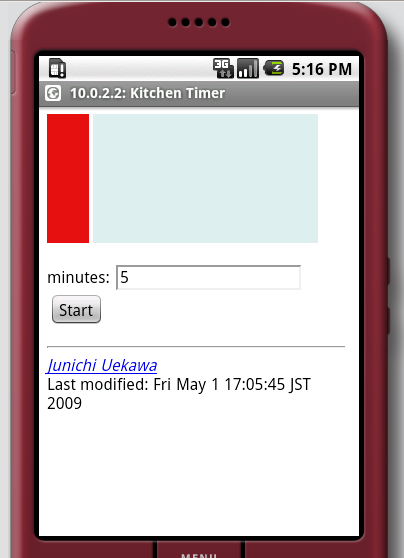
\includegraphics[width=0.3\hsize]{image200905/android-timer.png}

\subsection{Android$B$N4JC1$J%"%W%j%1!<%7%g%s$r:n@.$7$F5/F0$7$F$_$k(B}

$B$=$l$G$O!"(BAndroid $BMQ$N4JC1$J%"%W%j%1!<%7%g%s$r=q$$$F$_$^$7$g$&!#(B

\url{http://developer.android.com/guide/developing/eclipse-adt.html}
$B$K$7$?$,$C$FC8!9$H:n@.$7$^$9!#(B
$B$^$:!"(B
File$B$N(BNew Project $B$G(B Android $B$N$r%W%m%8%'%/%HA*Br$7$F:n@.$7$^$7$?!#(B
$B%?!<%2%C%H%S%k%I$O(B1.1$B$K$H$j$"$($:$7$m$H=q$$$F$"$j$^$9$,!"$h$/$o$+$i$J$$(B
$B$N$G!"<j85$N%U%!!<%`%&%'%"$N%P!<%8%g%s(B 1.5 $B$K$"$o$;$F$*$-$^$7$?!#(B

Run$B$N(BRun(Ctrl-F11)$B$G(BAndroid Application$B$rA*Br$9$k$H%(%_%e%l!<%?$r5/F0$7(B
$B$F%"%W%j%1!<%7%g%s$r<B9T$9$k$3$H$,$G$-$^$9!#(B
$B:G=i$K@8@.$5$l$?%=!<%9%3!<%I$N$^$^$N>uBV$@$H(B Hello World $B%"%W%j%1!<%7%g(B
$B%s$,5/F0$7$^$9!#(B

\subsection{Android$B$N4JC1$J%"%W%j%1!<%7%g%s$r=q$$$F$_$k(B}

$B%"%W%j%1!<%7%g%s$N:n@.$d%(%G%#%?$N5/F0$NItJ,$O$J$s$H$+$J$k$h$&$K$J$C$?$N(B
$B$G!"<!$O%A%e!<%H%j%"%k$rD/$a$F$_$^$9!#(B
Hello World$B$"$?$j$,$h$5$2$G$9!#(B

\url{http://developer.android.com/guide/tutorials/hello-world.html}

$B0lDL$jFI$s$G!"$H$j$"$($:%5%s%W%k$rD/$a$F$I$&$d$l$PJ8;zNs$rI=<($G$-$k$N$+(B
$B$r3NG'$7$?$N$G!"9%$-$JJ8;zNs$rI=<($9$k%"%W%j%1!<%7%g%s$r:n$C$F$_$^$9!#(B

Android $B$N(B top $B%3%^%s%I$G%W%m%;%9$N0lMw$r=PNO$G$-$k$N$G!"(B
$B%3%^%s%I$r<B9T$7$F$=$N=PNO$rI=<($9$k$@$1$N%"%W%j%1!<%7%g%s$r:n@.$7$F$_$^(B
$B$7$?!#(B
$BCf3K$r$J$9(Bsrc/jp.gr.netfort.dancer/TopView.java$B$O0J2<$N$h$&$K$J$j$^$7$?!#(B

\begin{commandline}
package jp.gr.netfort.dancer;

import android.app.Activity;
import android.os.Bundle;
import android.widget.TextView;
import java.io.*;

public class TopView extends Activity {
	/** Called when the activity is first created. */
	@Override
	public void onCreate(Bundle savedInstanceState) {
		super.onCreate(savedInstanceState);
		setContentView(R.layout.main);
		String [] command = { "top", "-n", "1"};
		String output = "";

		Runtime runtime = Runtime.getRuntime();
		Process process = null;
		try { 
			process = runtime.exec(command);
		} catch (Exception exception){
			System.exit(1);
		}
		BufferedReader reader = new BufferedReader(new InputStreamReader(process.getInputStream()));
		String line;
		try {
			while((line = reader.readLine()) != null) {
				output = output + line + "\n";
			}
		} catch (Exception exception) {
			System.exit(1);
		} finally {
			try {
				reader.close();
			} catch (Exception exception) {
				System.exit(1);
			}
		}
		TextView tv = new TextView(this);
		tv.setText(output);
		setContentView(tv);
	}
} 
\end{commandline}

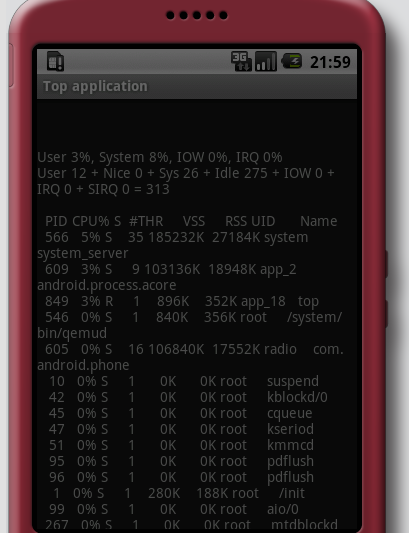
\includegraphics[width=0.3\hsize]{image200905/android-top.png}

\subsection{Android$B$N4JC1$J%"%W%j%1!<%7%g%s$r<B5!$G2TF/$5$;$F$_$k(B}

$B<B:]$K;H$&JXMx$J%"%W%j%1!<%7%g%s$r:n$C$F$_$^$7$g$&!#(B
$B%i%$%H%K%s%0%H!<%/$r<B;\$9$k:]$K$I$N%W%l%<%s%F!<%7%g%s$,5$$KF~$C$?$+$rI=(B
$BL@$9$k!"EjI<MQ$KMxMQ$9$k%\%?%s$G$b:n@.$7$^$7$g$&$+!#(B($BL$Dj(B)


\subsection{$B$*$^$1(B:$B%a%b%j>CHq$N@a8:(B}

$B<j85$N(BMacBook$B$K$O(B1GB$B$7$+%a%b%j$rEk:\$7$F$$$J$$$G$9!#(B
eclipse $B$O%G%U%)%k%H$N@_Dj$@$H5/F0$7$?=V4V$K(B1GB$B6a$/$N(B
$B2>A[%a%b%j$r>CHq$7!"B((BSwap$B$r;HMQ$7$F$7$^$&$H$$$&LdBj$,$"$j$^$7$?!#(B

\begin{commandline}
  PID USER      PR  NI  VIRT  RES  SHR S %CPU %MEM    TIME+  COMMAND            
17124 dancer    20   0  972m 302m  20m S    1 31.2   0:39.85 java
\end{commandline}

$B$H$j$"$($:!"%R%s%H$r5a$a$F(Bmaps$B$"$?$j$rD/$a$F$_$^$9!#(B
$B$=$l$J$j$K$?$/$5$s(Bmmap$B$7$F$$$^$9$,!"$=$l$@$1$G$O@bL@$G$-$J$$$h$&$J%a%b%j(B
$BNN0h$r3NJ]$7$F$$$^$9!#(B
\begin{commandline}
$ cat /proc/17124/status | grep Vm
VmPeak:	 1056748 kB
VmSize:	 1003316 kB
VmLck:	       0 kB
VmHWM:	  310740 kB
VmRSS:	  221616 kB
VmData:	  788504 kB
VmStk:	      84 kB
VmExe:	      36 kB
VmLib:	   38812 kB
VmPTE:	    1108 kB
$ cat /proc/17124/maps | grep rw | sort -rn -k5 
 .
\end{commandline}

$B$H$j$"$($:(BJava$B$N%"%W%j%1!<%7%g%s$N(BHeap$B$N;H$$J}$,$h$/$o$+$i$J$$$N$G!"(B
jconsole $B$G@\B3$7$FLdBj$r2r@O$7$^$9!#(B


$B%a%b%j%W!<%k$,$$$/$D$+$"$k$3$H$,$o$+$j$^$9!#(B

\begin{itemize}
 \item  Tenured Gen $B$,(B 60MB
 \item  Survivor 1MB
 \item  Code Cache $B$,(B 4MB
 \item  Perm Gen $B$,(B 70-90MB
 \item  Heap$B$O(B100MB(GC$B$7$?$i(B50MB$BDxEY(B)
\end{itemize}

eclipse.ini$B$,8=>u$3$&$J$C$F$$$k$N$G$9$,!"$3$l$r$*$=$k$*$=$k%A%e!<%K%s%0$7$F$_$^$9!#(B
\begin{commandline}
-showsplash
org.eclipse.platform
-framework
plugins/org.eclipse.osgi_3.4.2.R34x_v20080826-1230.jar
-vmargs
-Dosgi.requiredJavaVersion=1.5
-Xms40m
-Xmx256m
-XX:MaxPermSize=256m
\end{commandline}

$B5/F0;~$K3NJ]$7$?%R!<%W%a%b%j$NNN0h$r3+J|$7$F$$$J$$ItJ,$K$D$$$F$O!"(BGC$B$rIQ(B
$BHK$K9T$($P5/F0$O<c43CY$/$J$j$^$9$,$&$^$/$$$1$k$h$&$J5$$,$7$^$9!#(B
Xmx 128m$B$KJQ99$7$F$_$k$H!"<c43%a%b%j$N>CHq$,2<$,$j$^$7$?!#(B
$B$7$+$7$=$3$^$G7`E*$G$O$"$j$^$;$s$M!#(B
MaxPermSize$B$r(B64MB$B$K$9$k$H%(%i!<(B
\begin{commandline}
 Exception in thread "RMI TCP Connection(idle)" java.lang.OutOfMemoryError: PermGen space
\end{commandline}
$B$,H/@8$7$^$7$?!#(B
96MB$B$@$H%(%i!<$G$*$A$J$$$h$&$G$9!#(B

\begin{commandline}
  PID USER      PR  NI  VIRT  RES  SHR S %CPU %MEM    TIME+  $B%3%a%s%H(B
17124 dancer    20   0  972m 302m  20m S    1 31.2   0:39.85 java
19663 dancer    20   0  795m 296m  23m S    1 30.6   0:36.69 Heap 128MB$BHG(B
20266 dancer    20   0  661m 292m  22m S    1 30.1   0:41.62 MaxPermSize 96MB               
\end{commandline}

$B$,$s$P$C$F$_$?3d$K$O%a%b%j$,(B10MB$BDxEY$7$+@aLs$G$-$^$;$s$G$7$?!#(B
$B%(%_%e%l!<%?$b5/F0$7$F$$$k$H(B500MB$B$/$i$$(Bswap$B$K$$$C$F$7$^$&$N$G!"$D$i$$!#(B
$B%a%b%jGc$$$K$$$/$+$J!#(B

\begin{commandline}
-showsplash
org.eclipse.platform
-framework
plugins/org.eclipse.osgi_3.4.2.R34x_v20080826-1230.jar
-vmargs
-Dosgi.requiredJavaVersion=1.5
-Xms40m
-Xmx128m
-XX:MaxPermSize=96m
\end{commandline}


\subsection{$B;29MJ88%(B}

$BK\5-;v$N:n@.$K;29M$K$7$?J88%$G$9!#(B

\begin{itemize}
 \item \url{http://www.eclipse.org/}: eclipse
 \item \url{http://developer.android.com/}: Android $B$N%Z!<%8!"3+H/>pJs$,(B
       $B$^$H$^$C$F$$$k!#FC$K(B\url{http://developer.android.com/sdk/1.5_r1/index.html}: Android
       SDK 1.5$B$N%@%&%s%m!<%I%Z!<%8$+$i$?$I$k%Z!<%8$,=EMW!#(B
 \item
      \url{http://developer.android.com/guide/basics/what-is-android.html}: 
      SDK$B$N3+H/%^%K%e%"%k!#(B
      SDK $B$N(B\url{./android-sdk-linux_x86-1.5_r1/docs/}$B$KF1$8$b$N$,$"$k$N(B
      $B$G%*%U%i%$%s$G$b0B?4!#(B
      $B$?$@$7%*%s%i%$%s$N%I%-%e%a%s%H$OHyL/$JD{@5$,%"%C%W%G!<%H$5$lB3$1$F(B
      $B$$$k$h$&$J$N$G%M%C%H%o!<%/@\B3$,MxMQ$G$-$k%*%s%i%$%s$N>l9g$O$=$A$i(B
      $B$r;2>H$9$k$[$&$,$h$$$+$b$7$l$^$;$s!#(B
\end{itemize}

\clearpage

%\printindex

\cleartooddpage

\vspace*{15cm}
\hrule
\vspace{2mm}

\includegraphics[width=2cm]{image200502/openlogo-nd.eps}
\noindent \Large \bf Debian $BJY6/2q;qNA(B\\ \\
\noindent \normalfont \debmtgyear{}$BG/(B\debmtgmonth{}$B7n(B\debmtgdate{}$BF|(B \hspace{5mm}  $B=iHGBh(B1$B:~H/9T(B\\
\noindent \normalfont $BEl5~%(%j%"(B Debian $BJY6/2q(B $B!JJT=8!&0u:~!&H/9T!K(B\\
\hrule


\end{document}
